\subsection{2D time-dependent Stokes sphere with deformable free surface}\label{sec:sphere}
This experiment is performed in a unit square domain with the gravity acceleration fixed to $g_y=-1$. The sphere has $\rho_s=2$ and $\eta_s=10^3$ and is
initially centred at ($0.5;0.6$) with radius $R=0.123456789$. The fluid surrounding the sphere has $\rho_f=1$ and $\eta_f=1$ and occupies the domain for
$y\leq 0.75$, while for $y>0.75$ the air has $\rho_a=0$ and $\eta_a=10^{-3}$. Velocity boundary conditions are set to free slip on all sides. The Courant
number is set to 0.25. The experiments run for 200 s using grid resolutions from $150\times150$ to $512\times512$ elements, with 25 randomly distributed markers
per element, and for different average schemes for the viscosity. The interface between the fluid and the air is tracked by means of the markers chain. Results
in terms of velocity and pressure fields and topography variations are compared with results obtained with ASPECT
\citep{Kronbichler2012,Heister2017,Bangerth2020,Bangerth2020a} and they can be found at
\url{https://github.com/cedrict/fieldstone/tree/master/images/stokes_sphere_fs2D} and
\url{https://github.com/aleregorda/Benchmarks/tree/main/Surface_processes/Time_dependent_sphere}. Results in terms of the $v_{\textrm{rms}}$ in case of 
an arithmetic average are also shown in Fig. \ref{fig:inst_spherefs}.

\begin{figure}
\centering
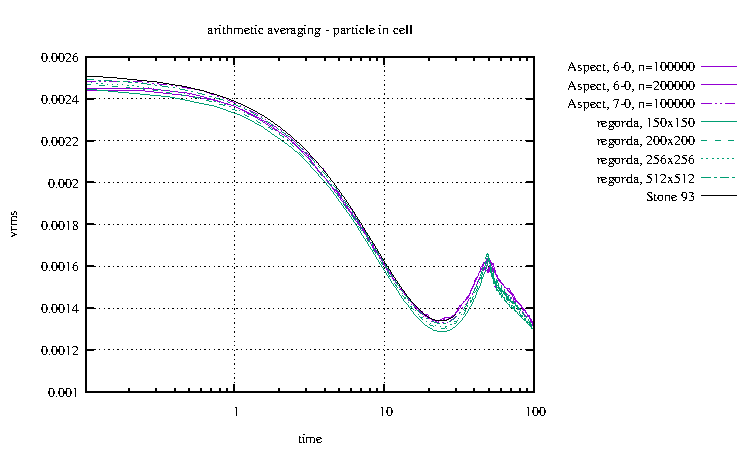
\includegraphics[width=400px]{./Figures/vrms_arithm.pdf}
\caption{$v_{\textrm{rms}}$ for different grid resolutions as function of time for the 2D time-dependent Stokes sphere experiment in case of an arithmetic average.
Results are compared with results obtained by ASPECT.}
\label{fig:inst_spherefs}
\end{figure}